%\subsection{تخمین پارامتر کانال‌های رول-پیچ}
%برای اصلاح پارامترها رول-پیچ چندین آزمایش انجام شد و با استفاده از داده‌های ثبت شده از وضعیت استند در کانال رول-پپچ و جعبه‌ابزار
%\lr{Parameter Estimator}
%پارامترهای کانال رول-پیچ اصلاح شدند.
%برای آزمایش تمامی موتورها با دور مختلف شروع به حرکت کردند و از خروجی سنسور داده برداری شد. سپس، مدل و  داده‌های ثبت شده سنسور (وضعیت استند در کانال رول-پیج)  به جعبه‌ابزار
%\lr{Parameter Estimator}
%داده شد. وضعیت کانال رول-پیچ استند در شبیه‌سازی و واقعیت بعد از اصلاح پارامترهای کانال‌ رول-پیچ بعد در شکل‌های
%(\ref{roll_pitch_ps1}, \ref{roll_pitch_ps2}, \ref{roll_pitch_ps3}, \ref{roll_pitch_ps4}, \ref{roll_pitch_ps5}, \ref{roll_pitch_ps6}, \ref{roll_pitch_ps7})
%آورده شده است.

%\begin{figure}[H]
%	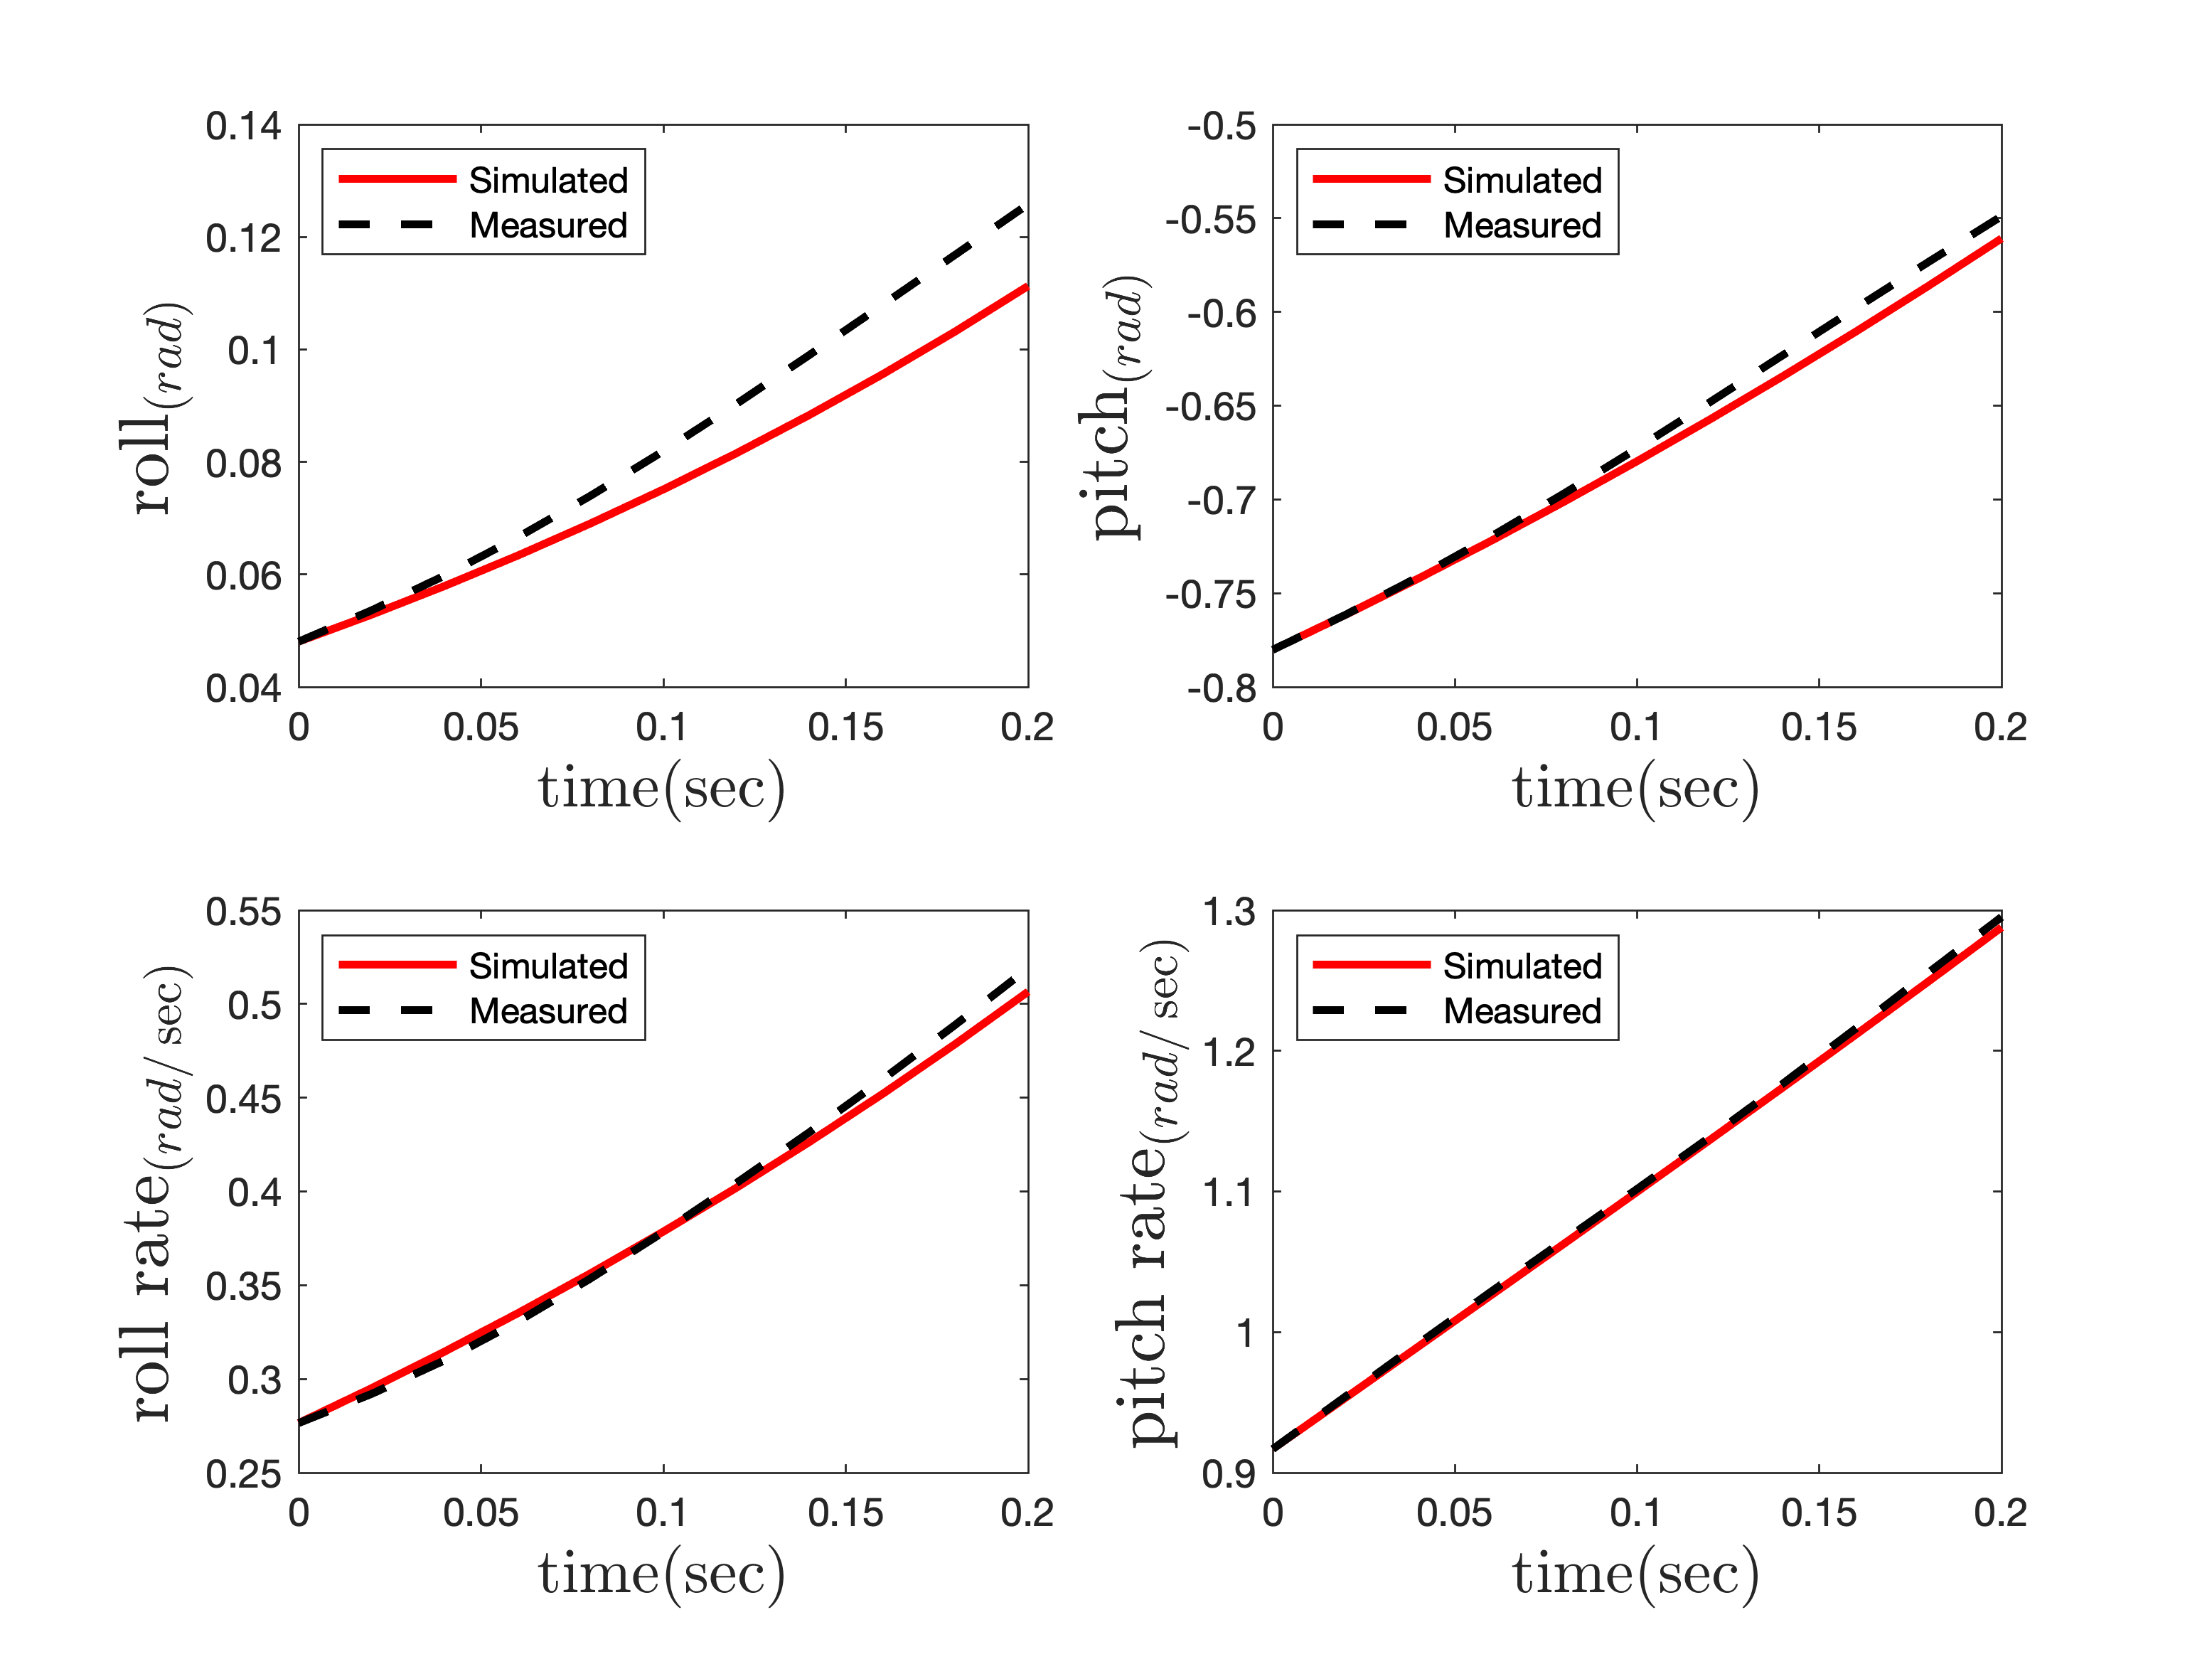
\includegraphics[width=12cm]{../Figures/RCP/roll_pitch_parameter_estimation/RCP_roll_pitch_S1.png}
%	\centering
%	\caption{مقايسه وضعیت استند در  آزمايش اول و شبیه‌سازی، پس از تخمین پارامترهای کانال رول-پیچ}
%	\label{roll_pitch_ps1}
%\end{figure}
%\begin{figure}[H]
%	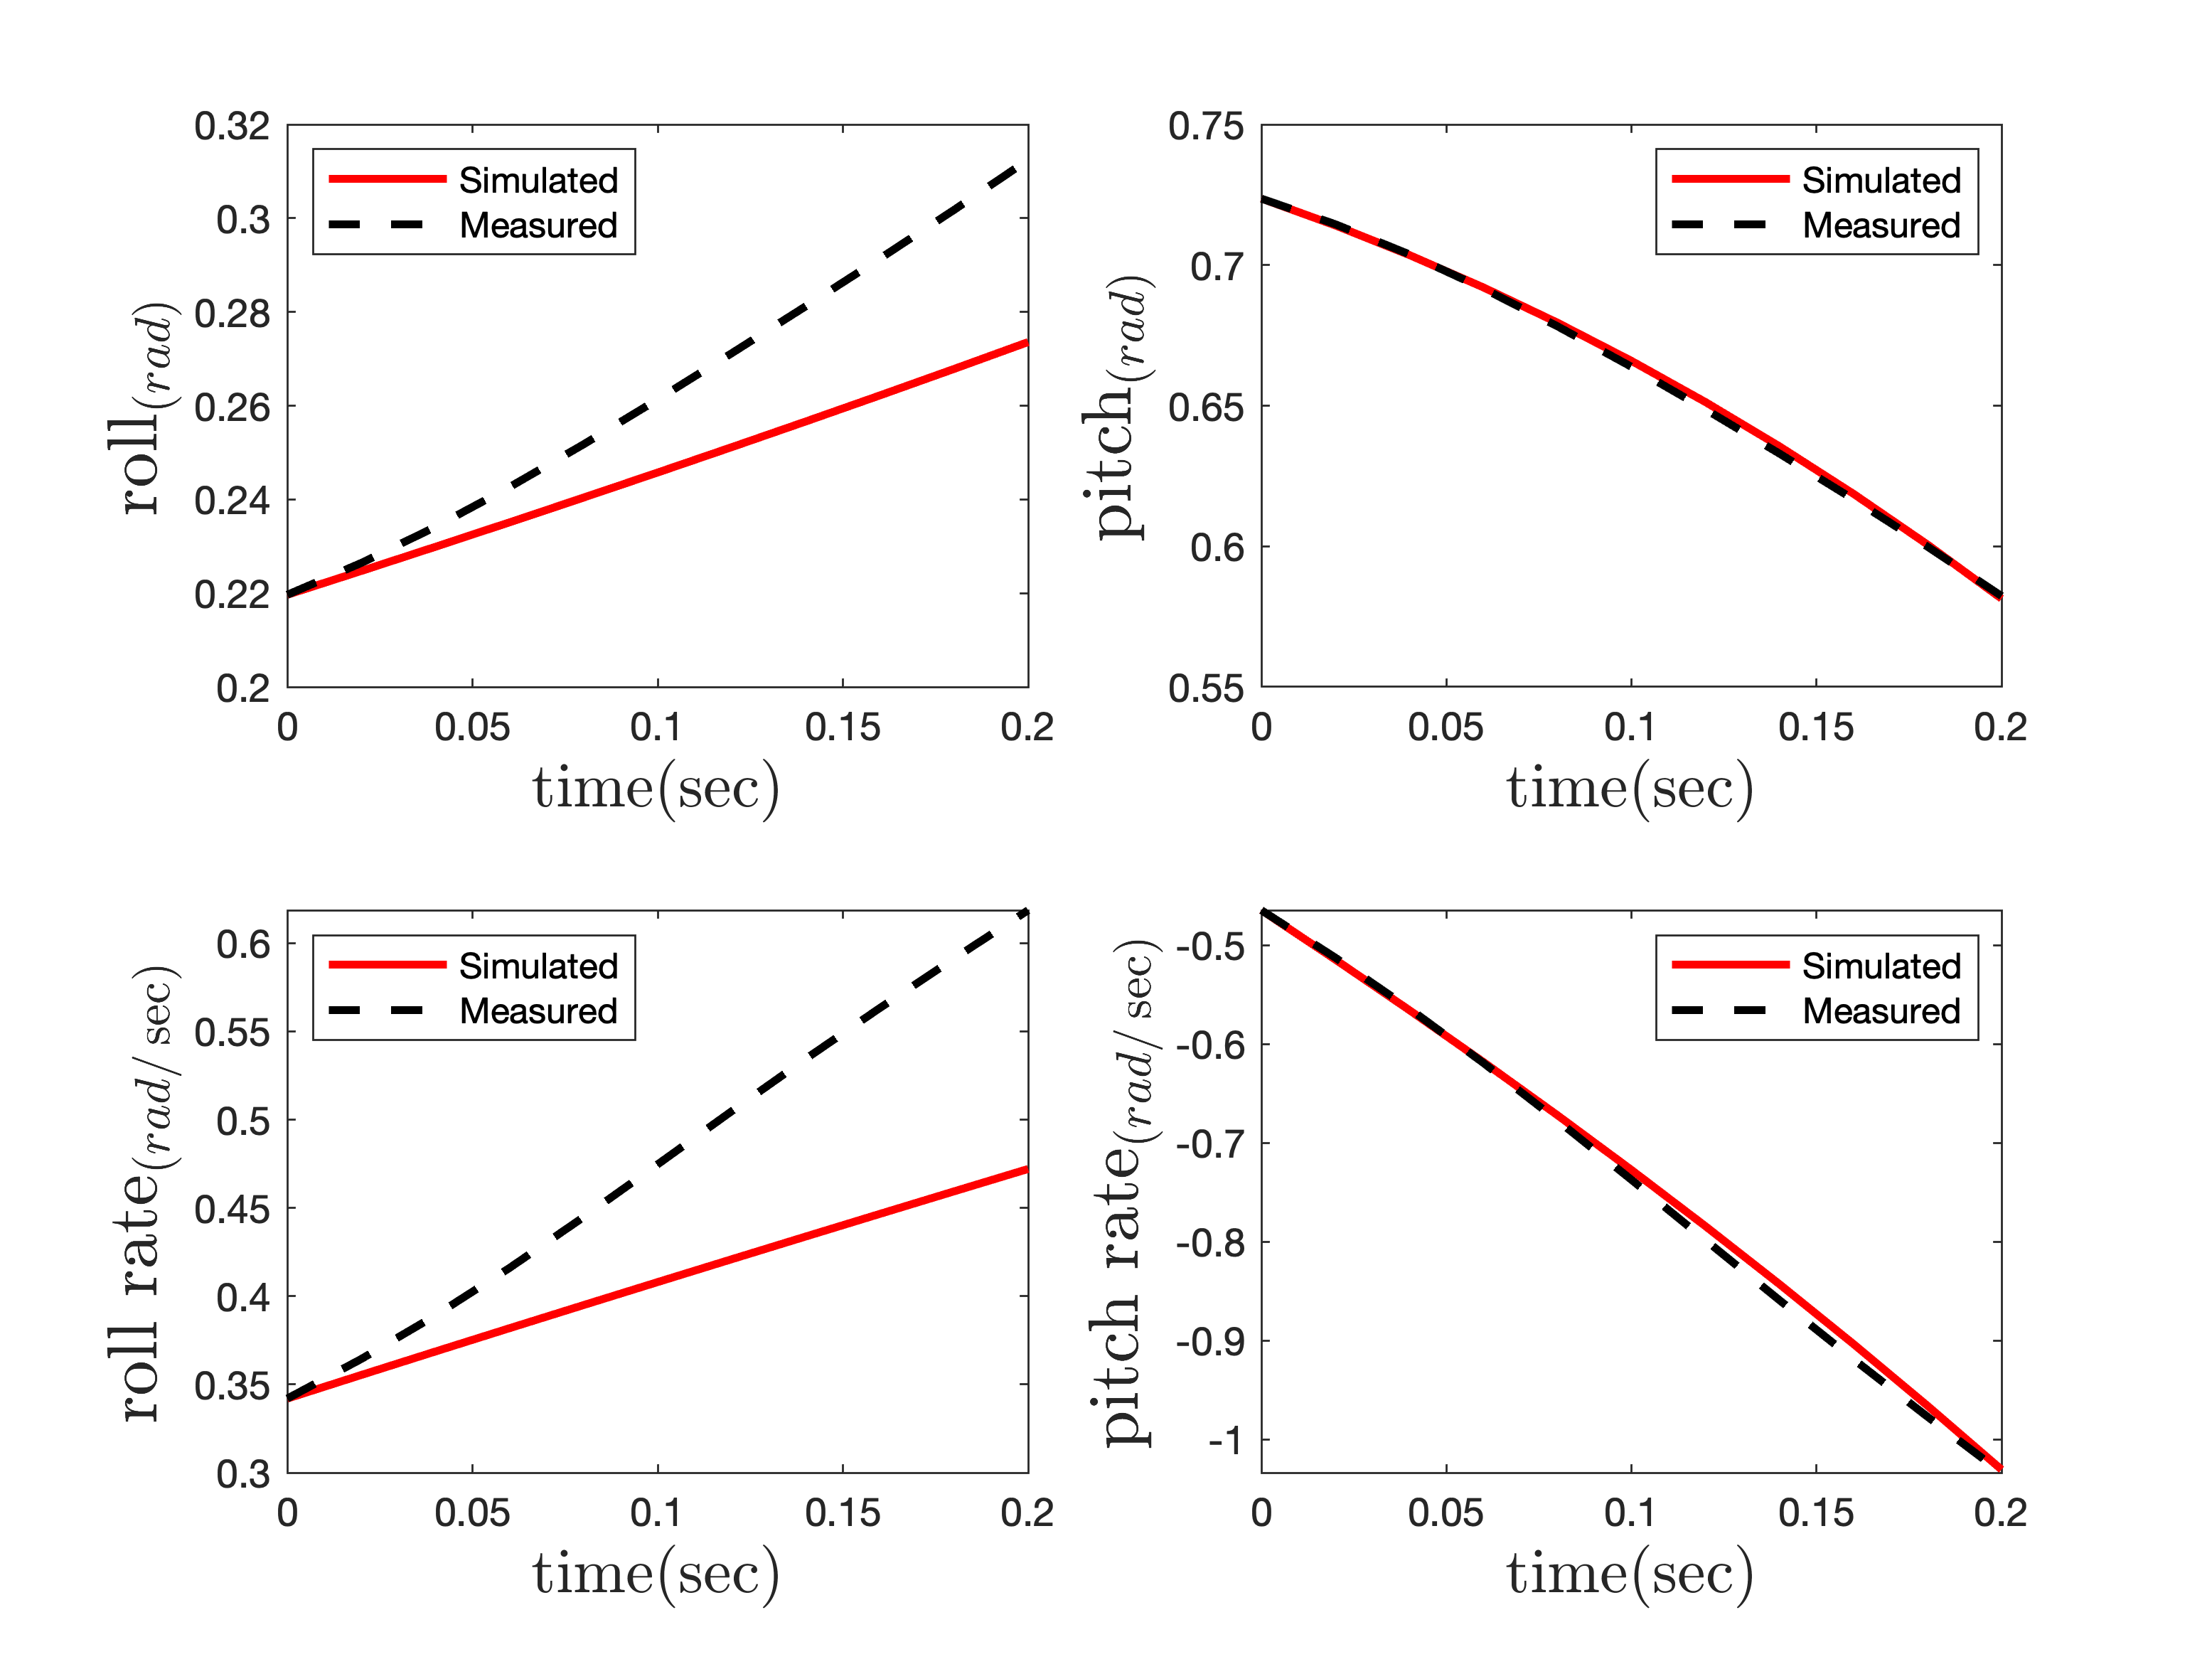
\includegraphics[width=12cm]{../Figures/RCP/roll_pitch_parameter_estimation/RCP_roll_pitch_S2.png}
%	\centering
%	\caption{مقايسه وضعیت استند در  آزمايش دوم و شبیه‌سازی، پس از تخمین پارامترهای کانال رول-پیچ}
%	\label{roll_pitch_ps2}
%\end{figure}
%\begin{figure}[H]
%	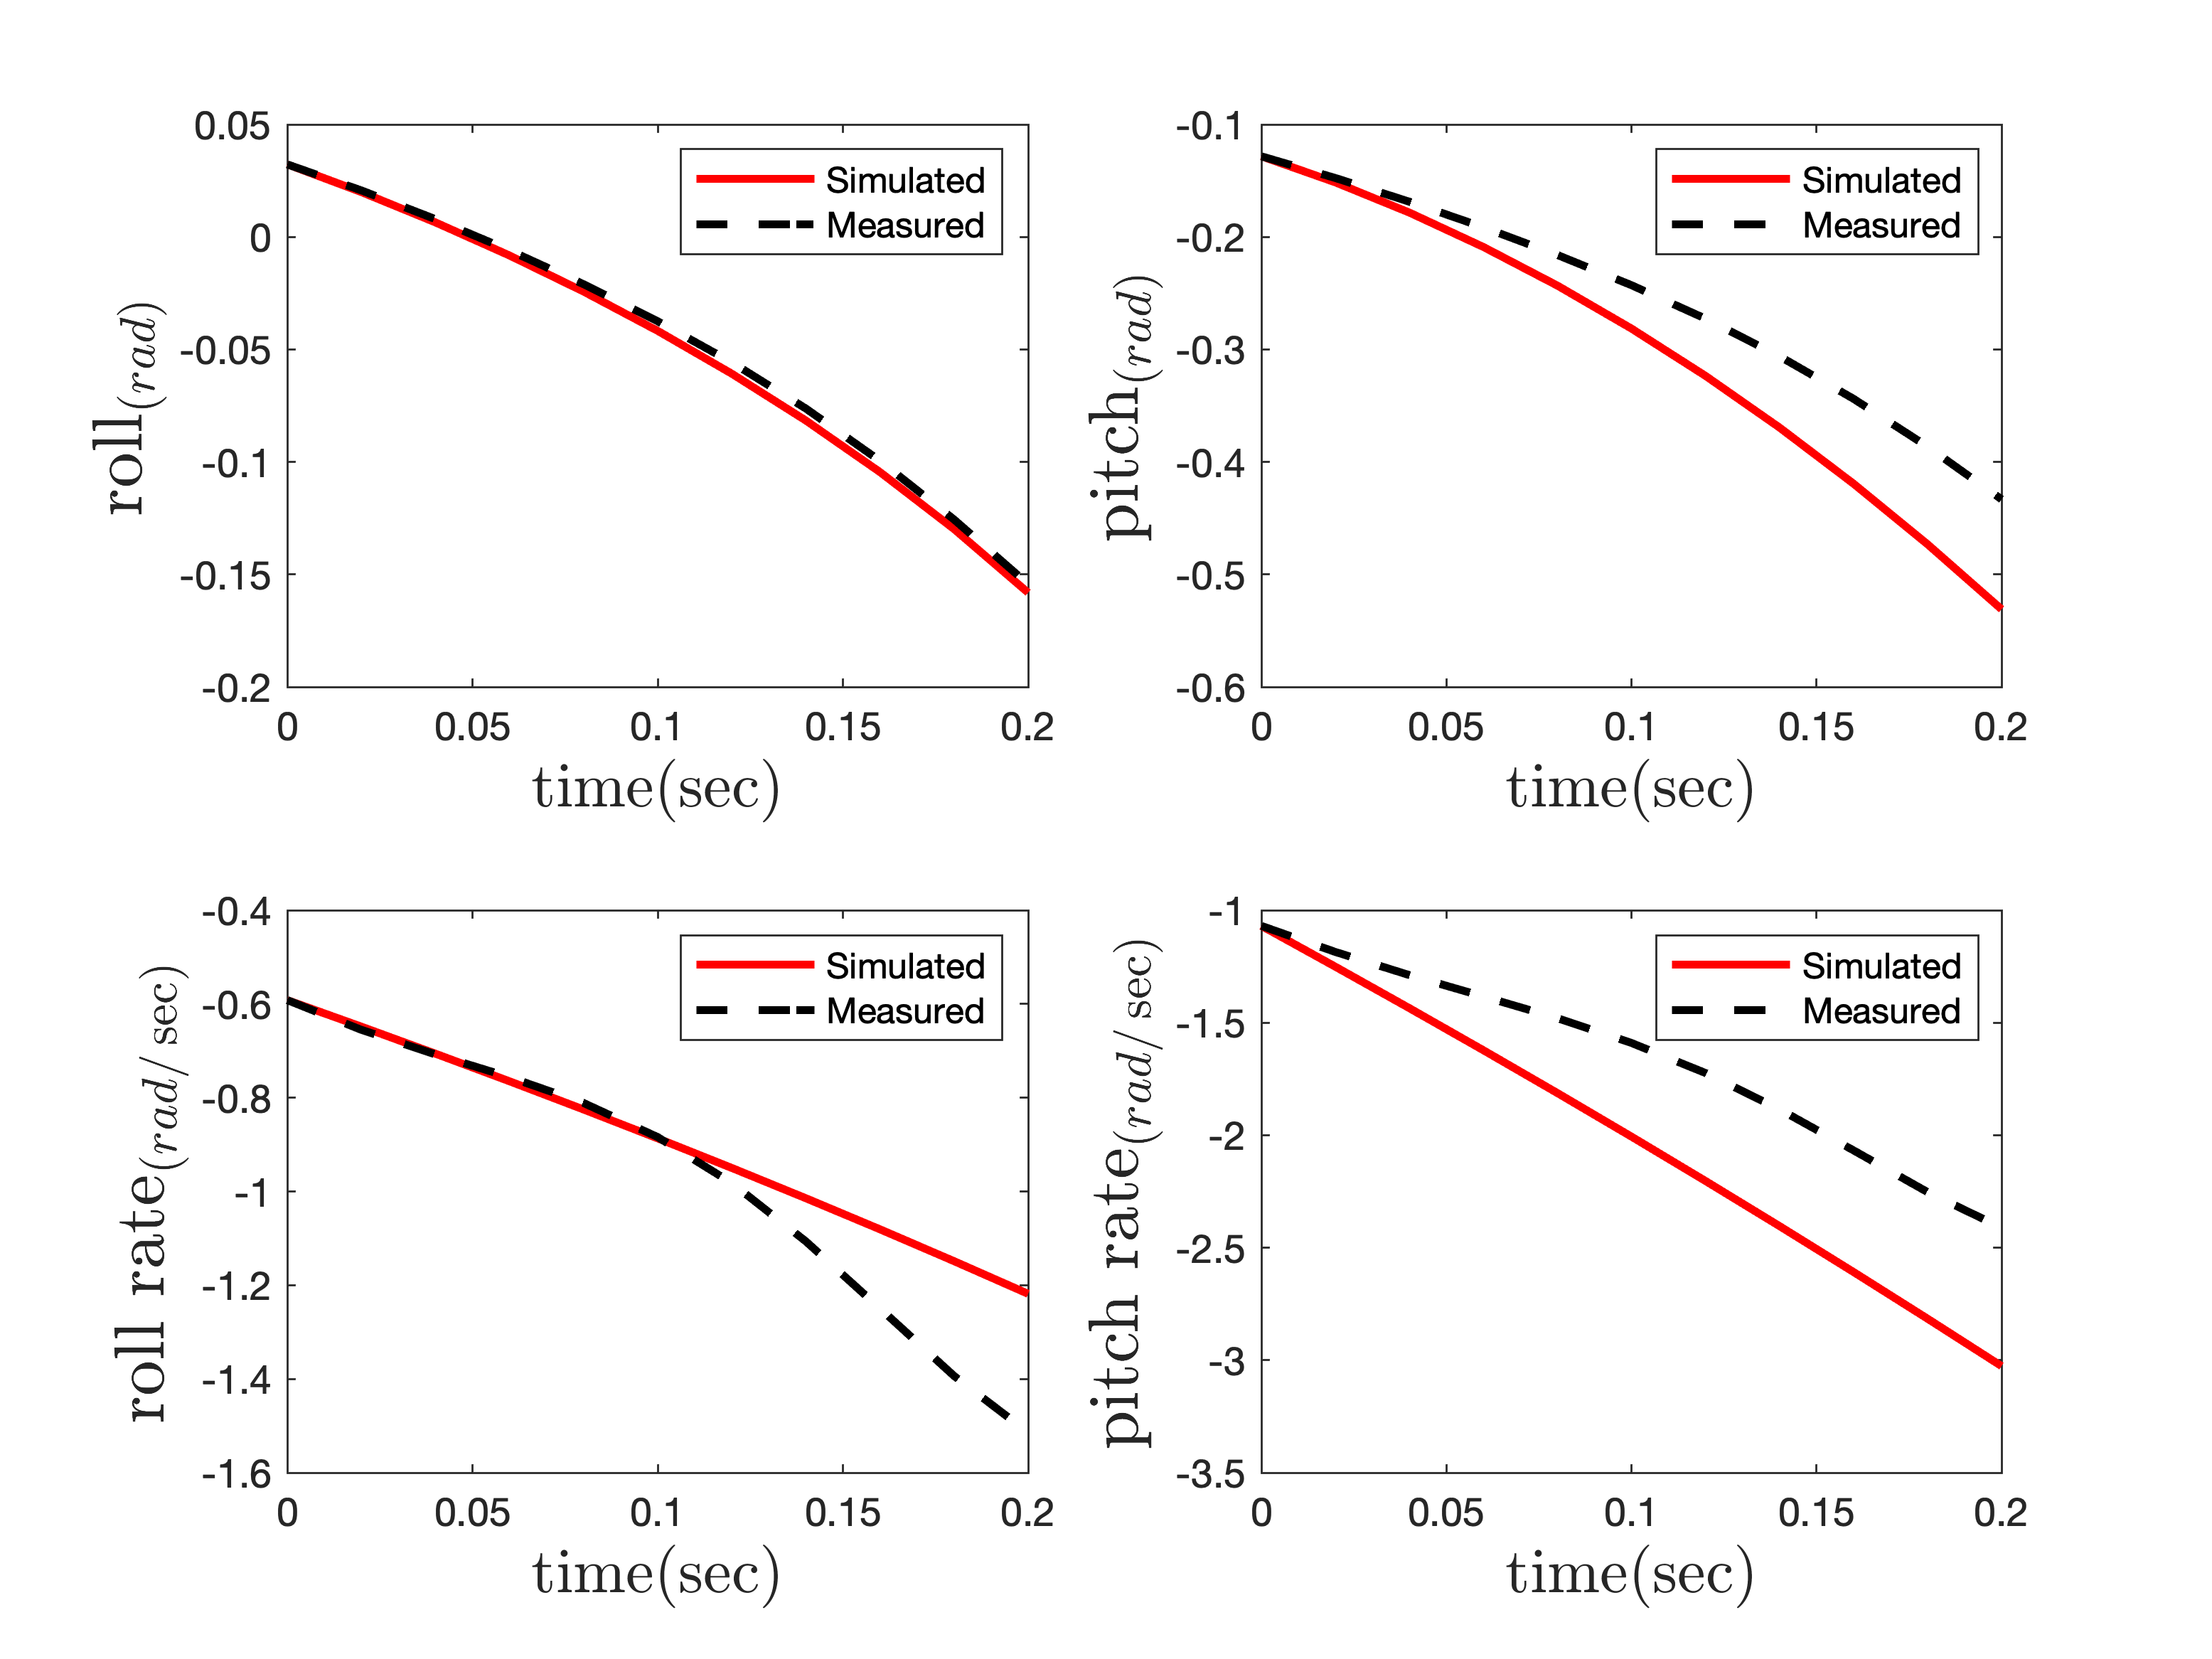
\includegraphics[width=12cm]{../Figures/RCP/roll_pitch_parameter_estimation/RCP_roll_pitch_S3.png}
%	\centering
%	\caption{مقايسه وضعیت استند در  آزمايش سوم و شبیه‌سازی، پس از تخمین پارامترهای کانال رول-پیچ}
%	\label{roll_pitch_ps3}
%\end{figure}
%\begin{figure}[H]
%	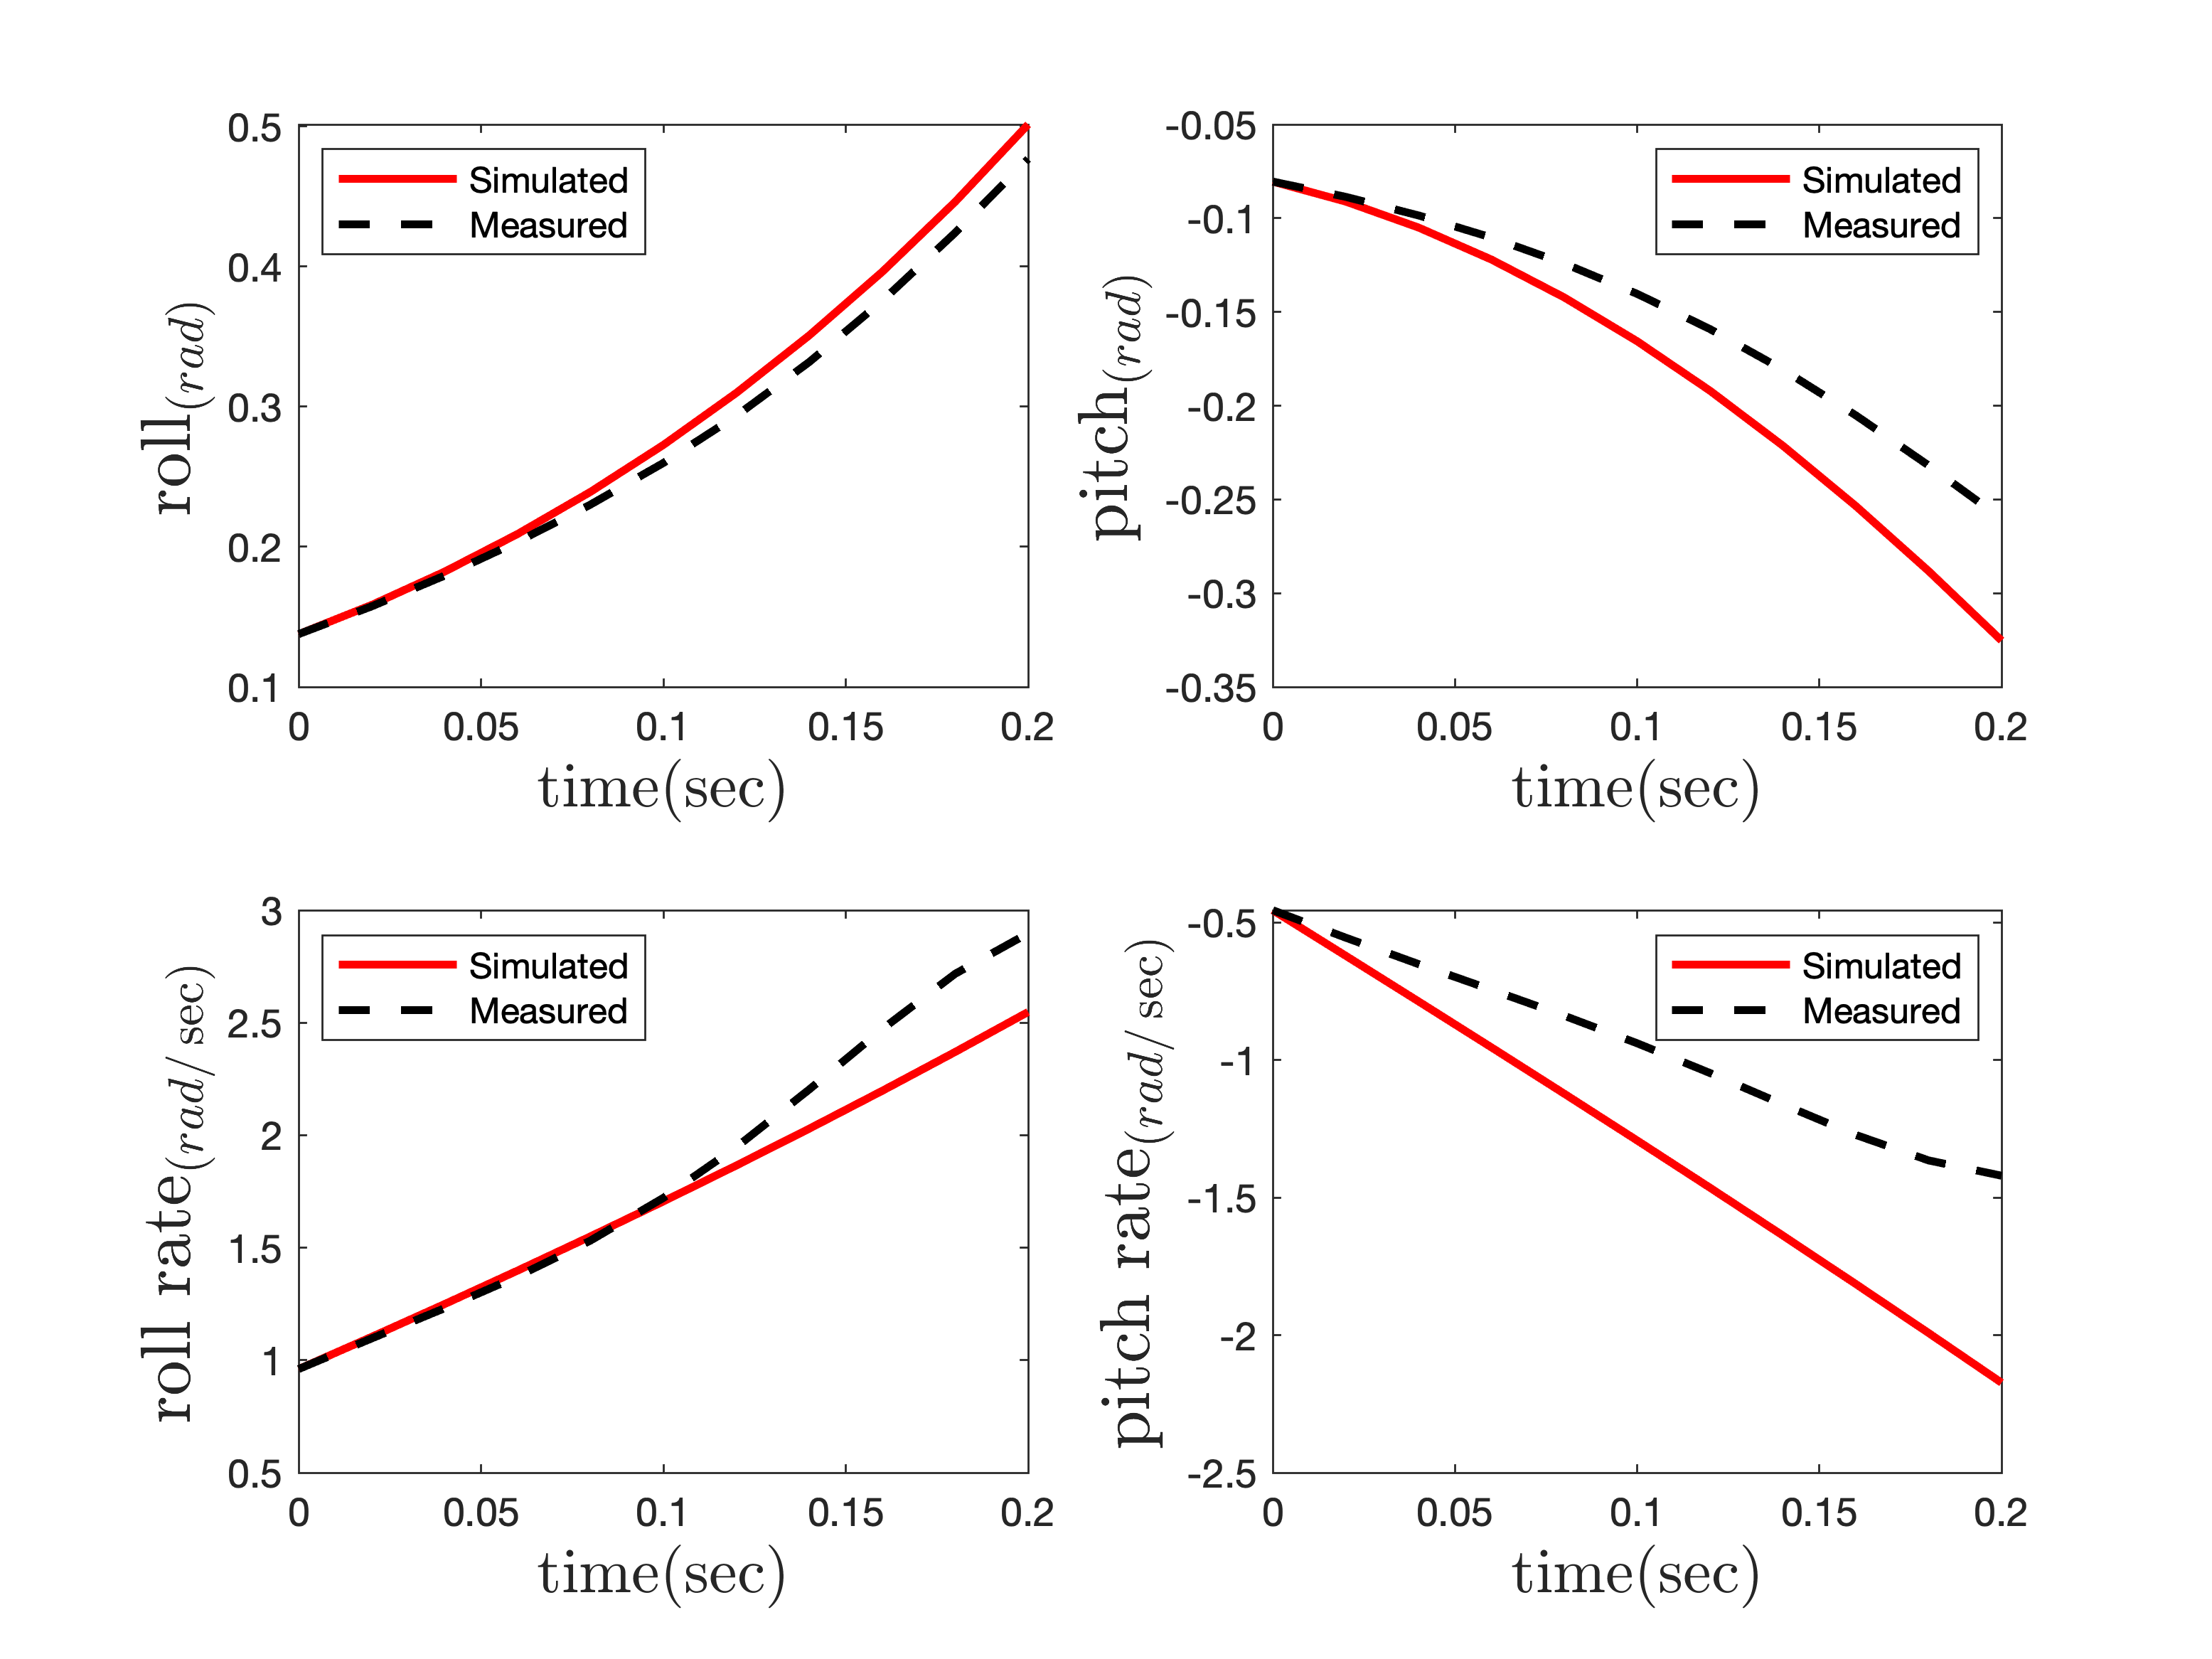
\includegraphics[width=12cm]{../Figures/RCP/roll_pitch_parameter_estimation/RCP_roll_pitch_S4.png}
%	\centering
%	\caption{مقايسه وضعیت استند در  آزمايش چهارم و شبیه‌سازی، پس از تخمین پارامترهای کانال رول-پیچ}
%	\label{roll_pitch_ps4}
%\end{figure}
%\begin{figure}[H]
%	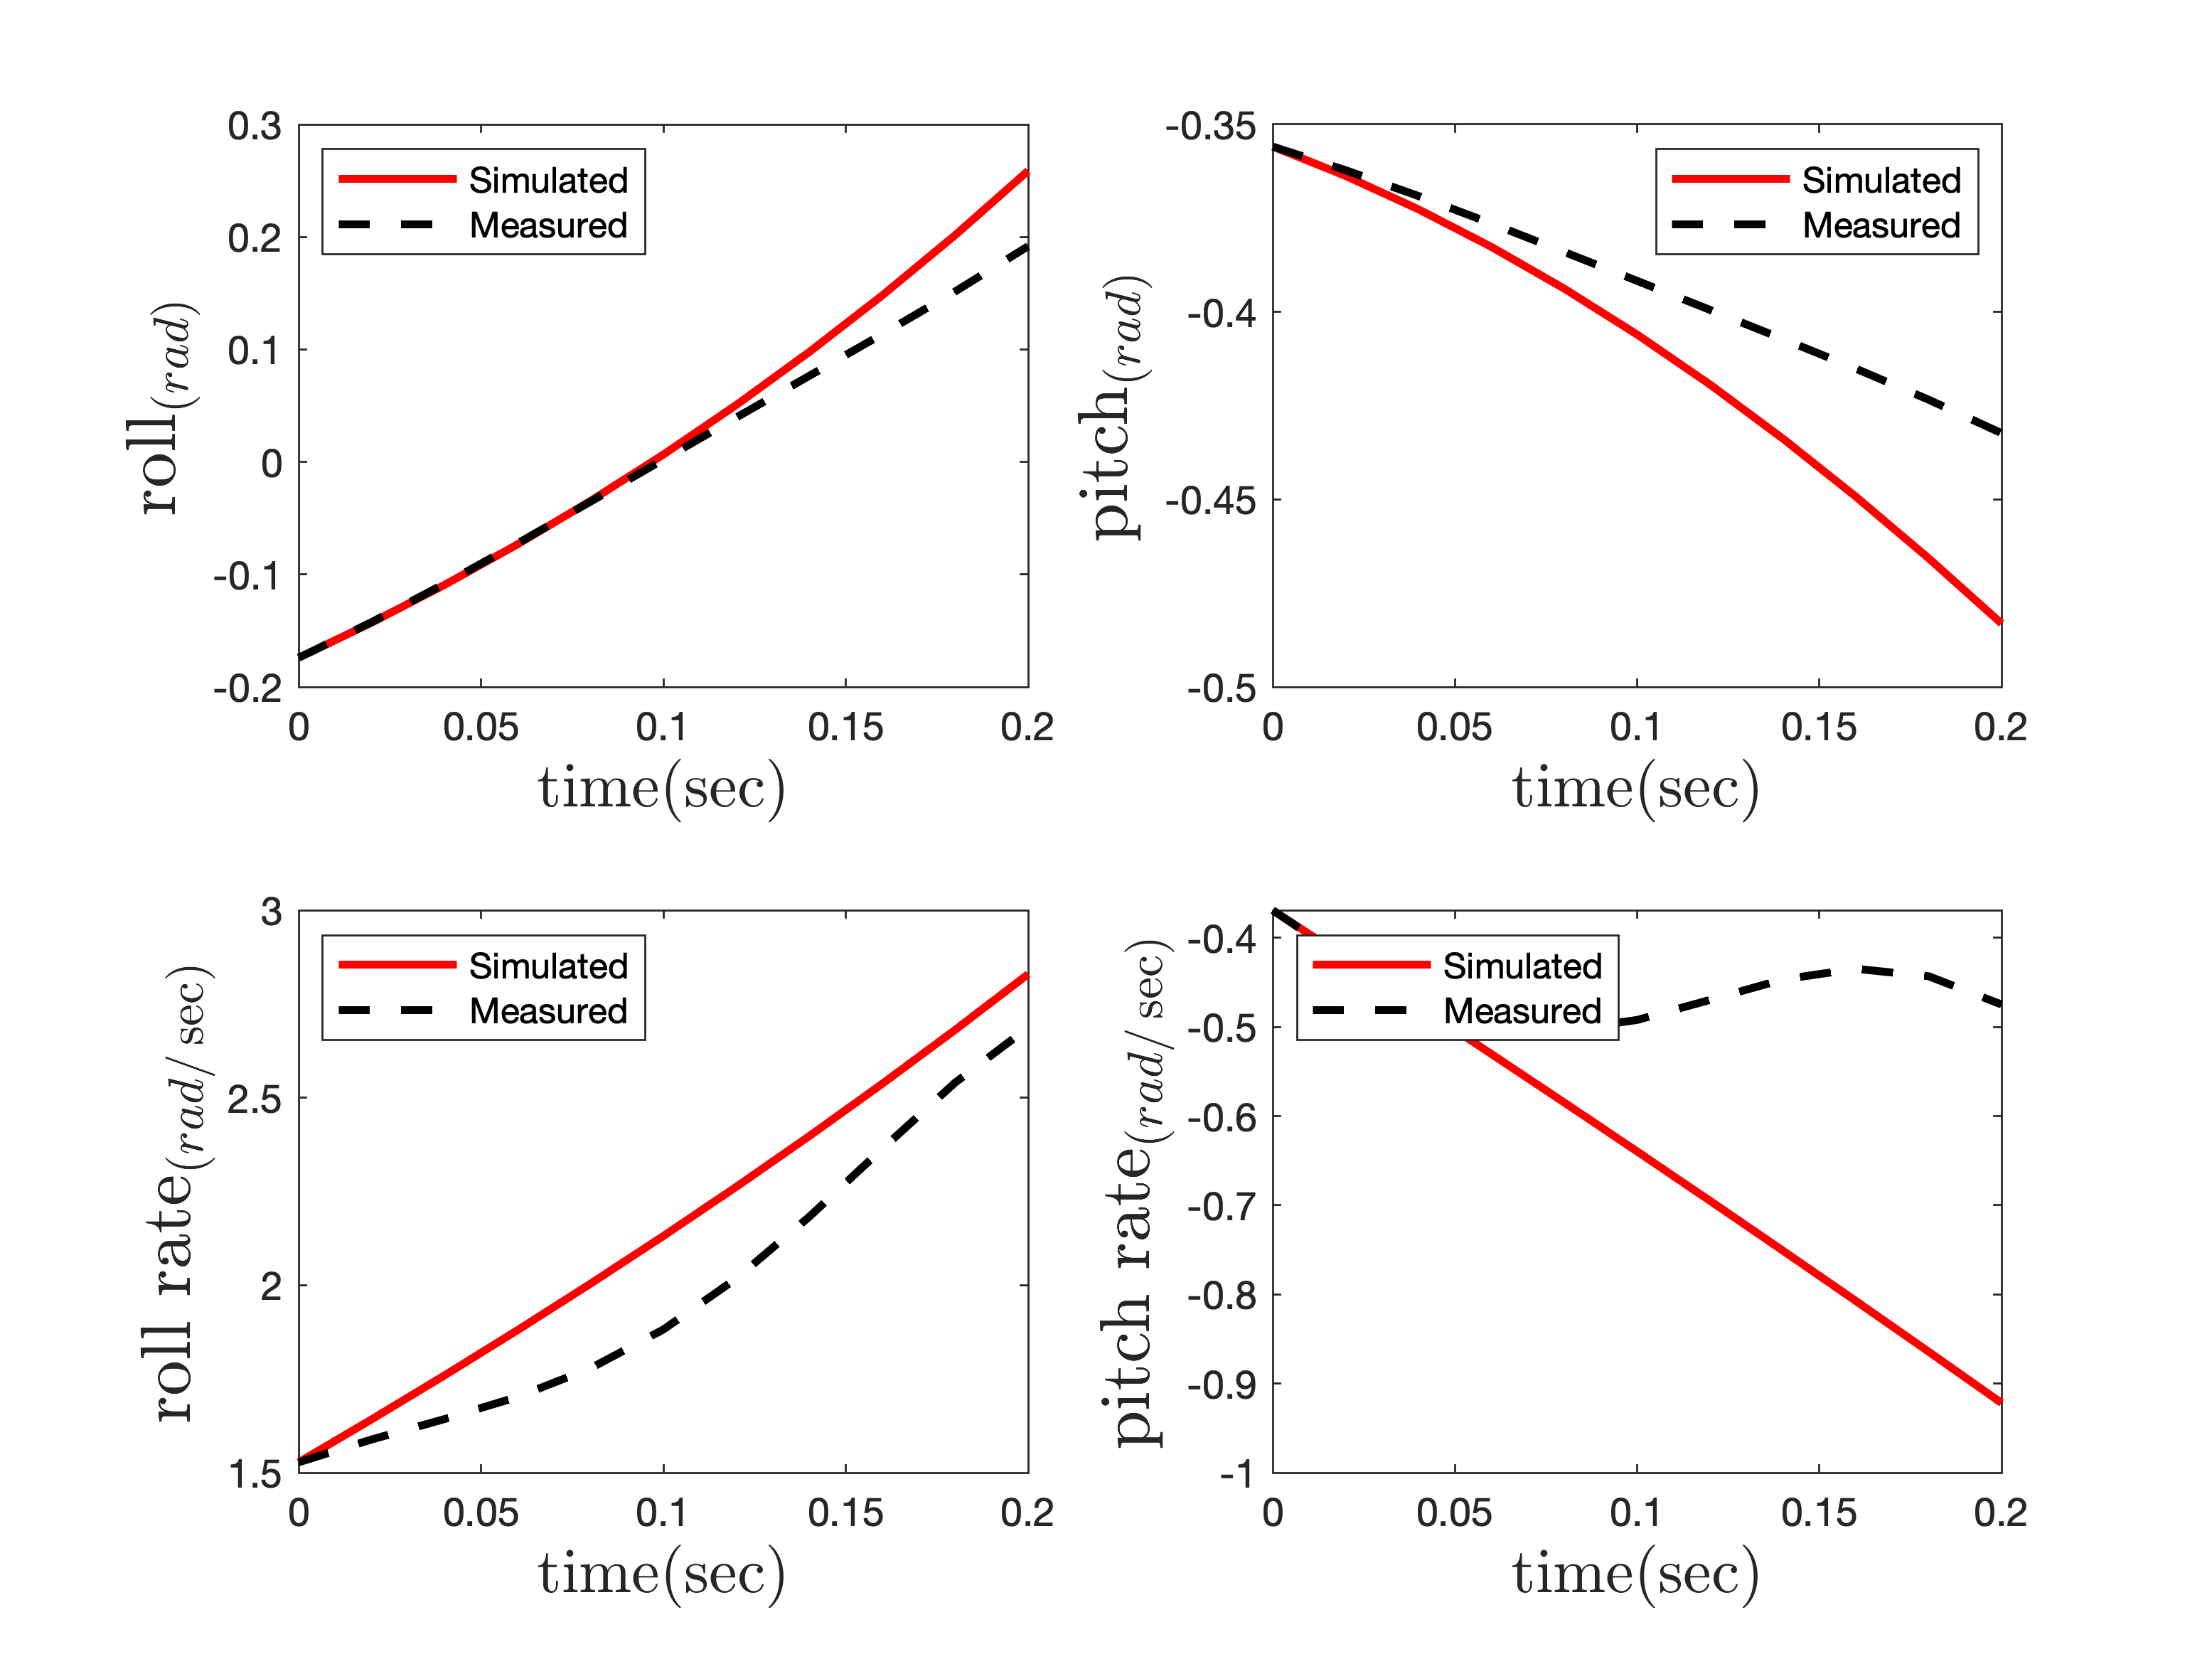
\includegraphics[width=12cm]{../Figures/RCP/roll_pitch_parameter_estimation/RCP_roll_pitch_S5.png}
%	\centering
%	\caption{مقايسه وضعیت استند در  آزمايش پنجم و شبیه‌سازی، پس از تخمین پارامترهای کانال رول-پیچ}
%	\label{roll_pitch_ps5}
%\end{figure}
%\begin{figure}[H]
%	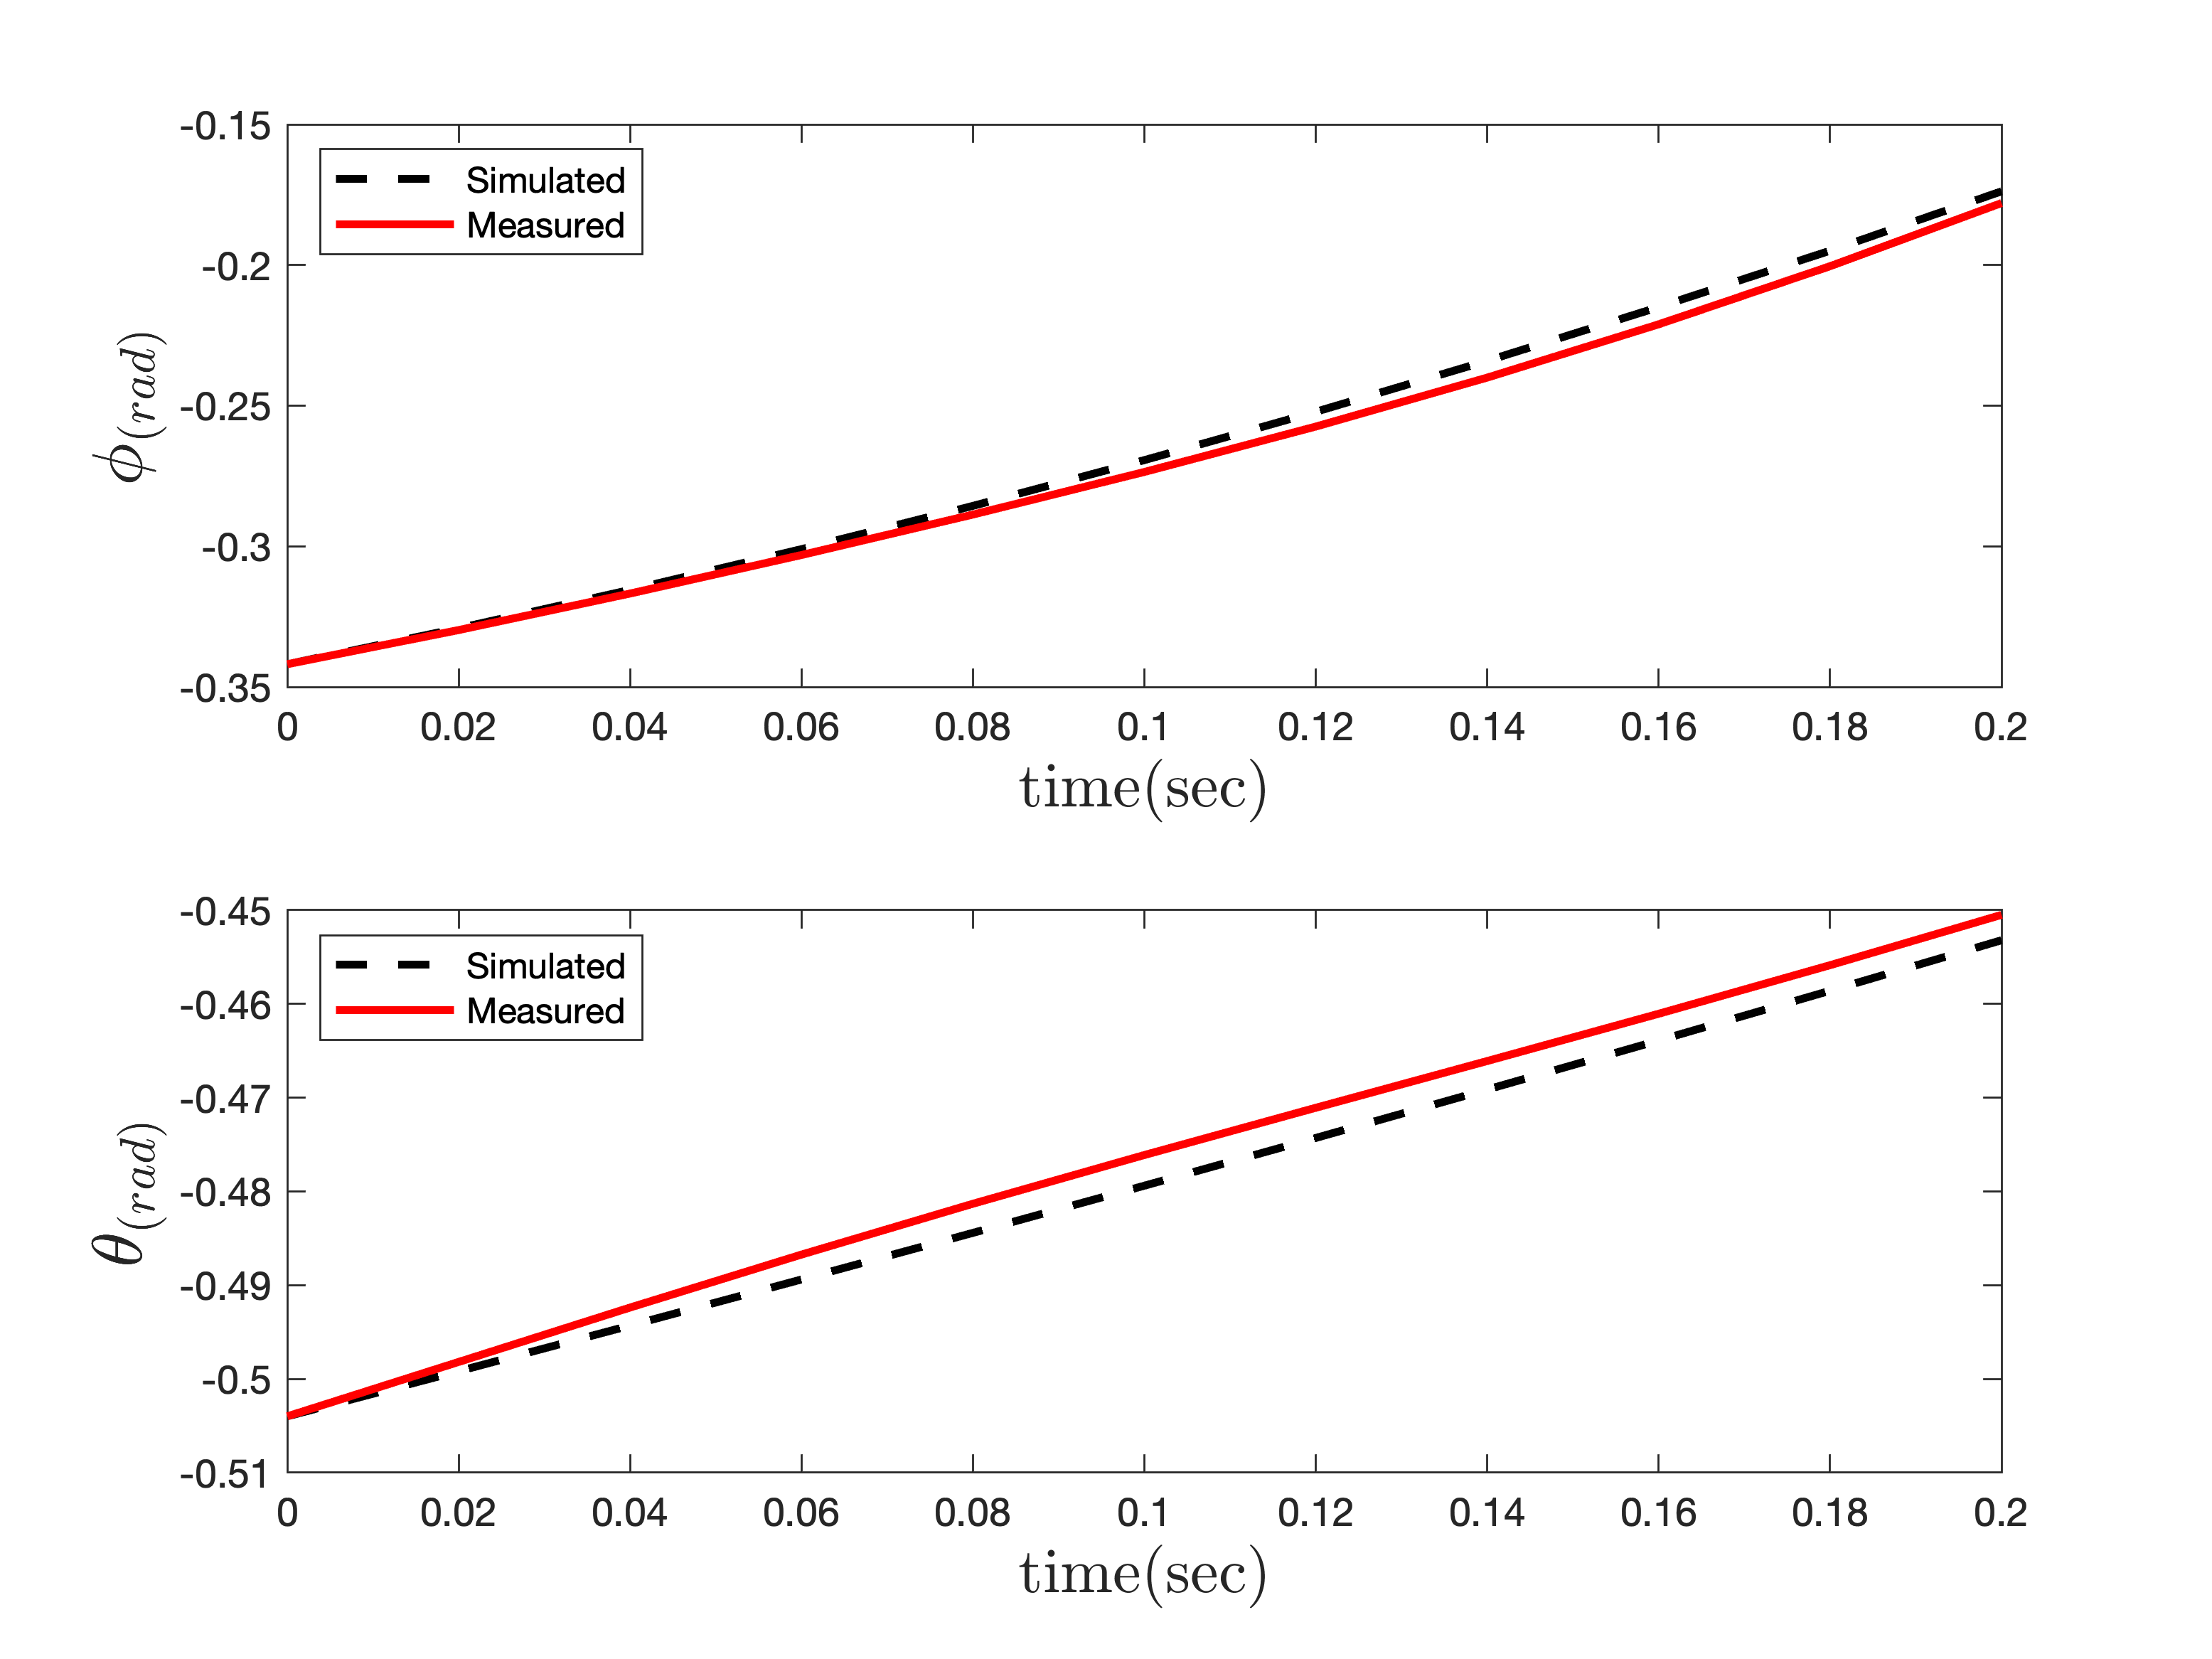
\includegraphics[width=12cm]{../Figures/RCP/roll_pitch_parameter_estimation/RCP_roll_pitch_S6.png}
%	\centering
%	\caption{مقايسه وضعیت استند در  آزمايش ششم و شبیه‌سازی، پس از تخمین پارامترهای کانال رول-پیچ}
%	\label{roll_pitch_ps6}
%\end{figure}
%\begin{figure}[H]
%	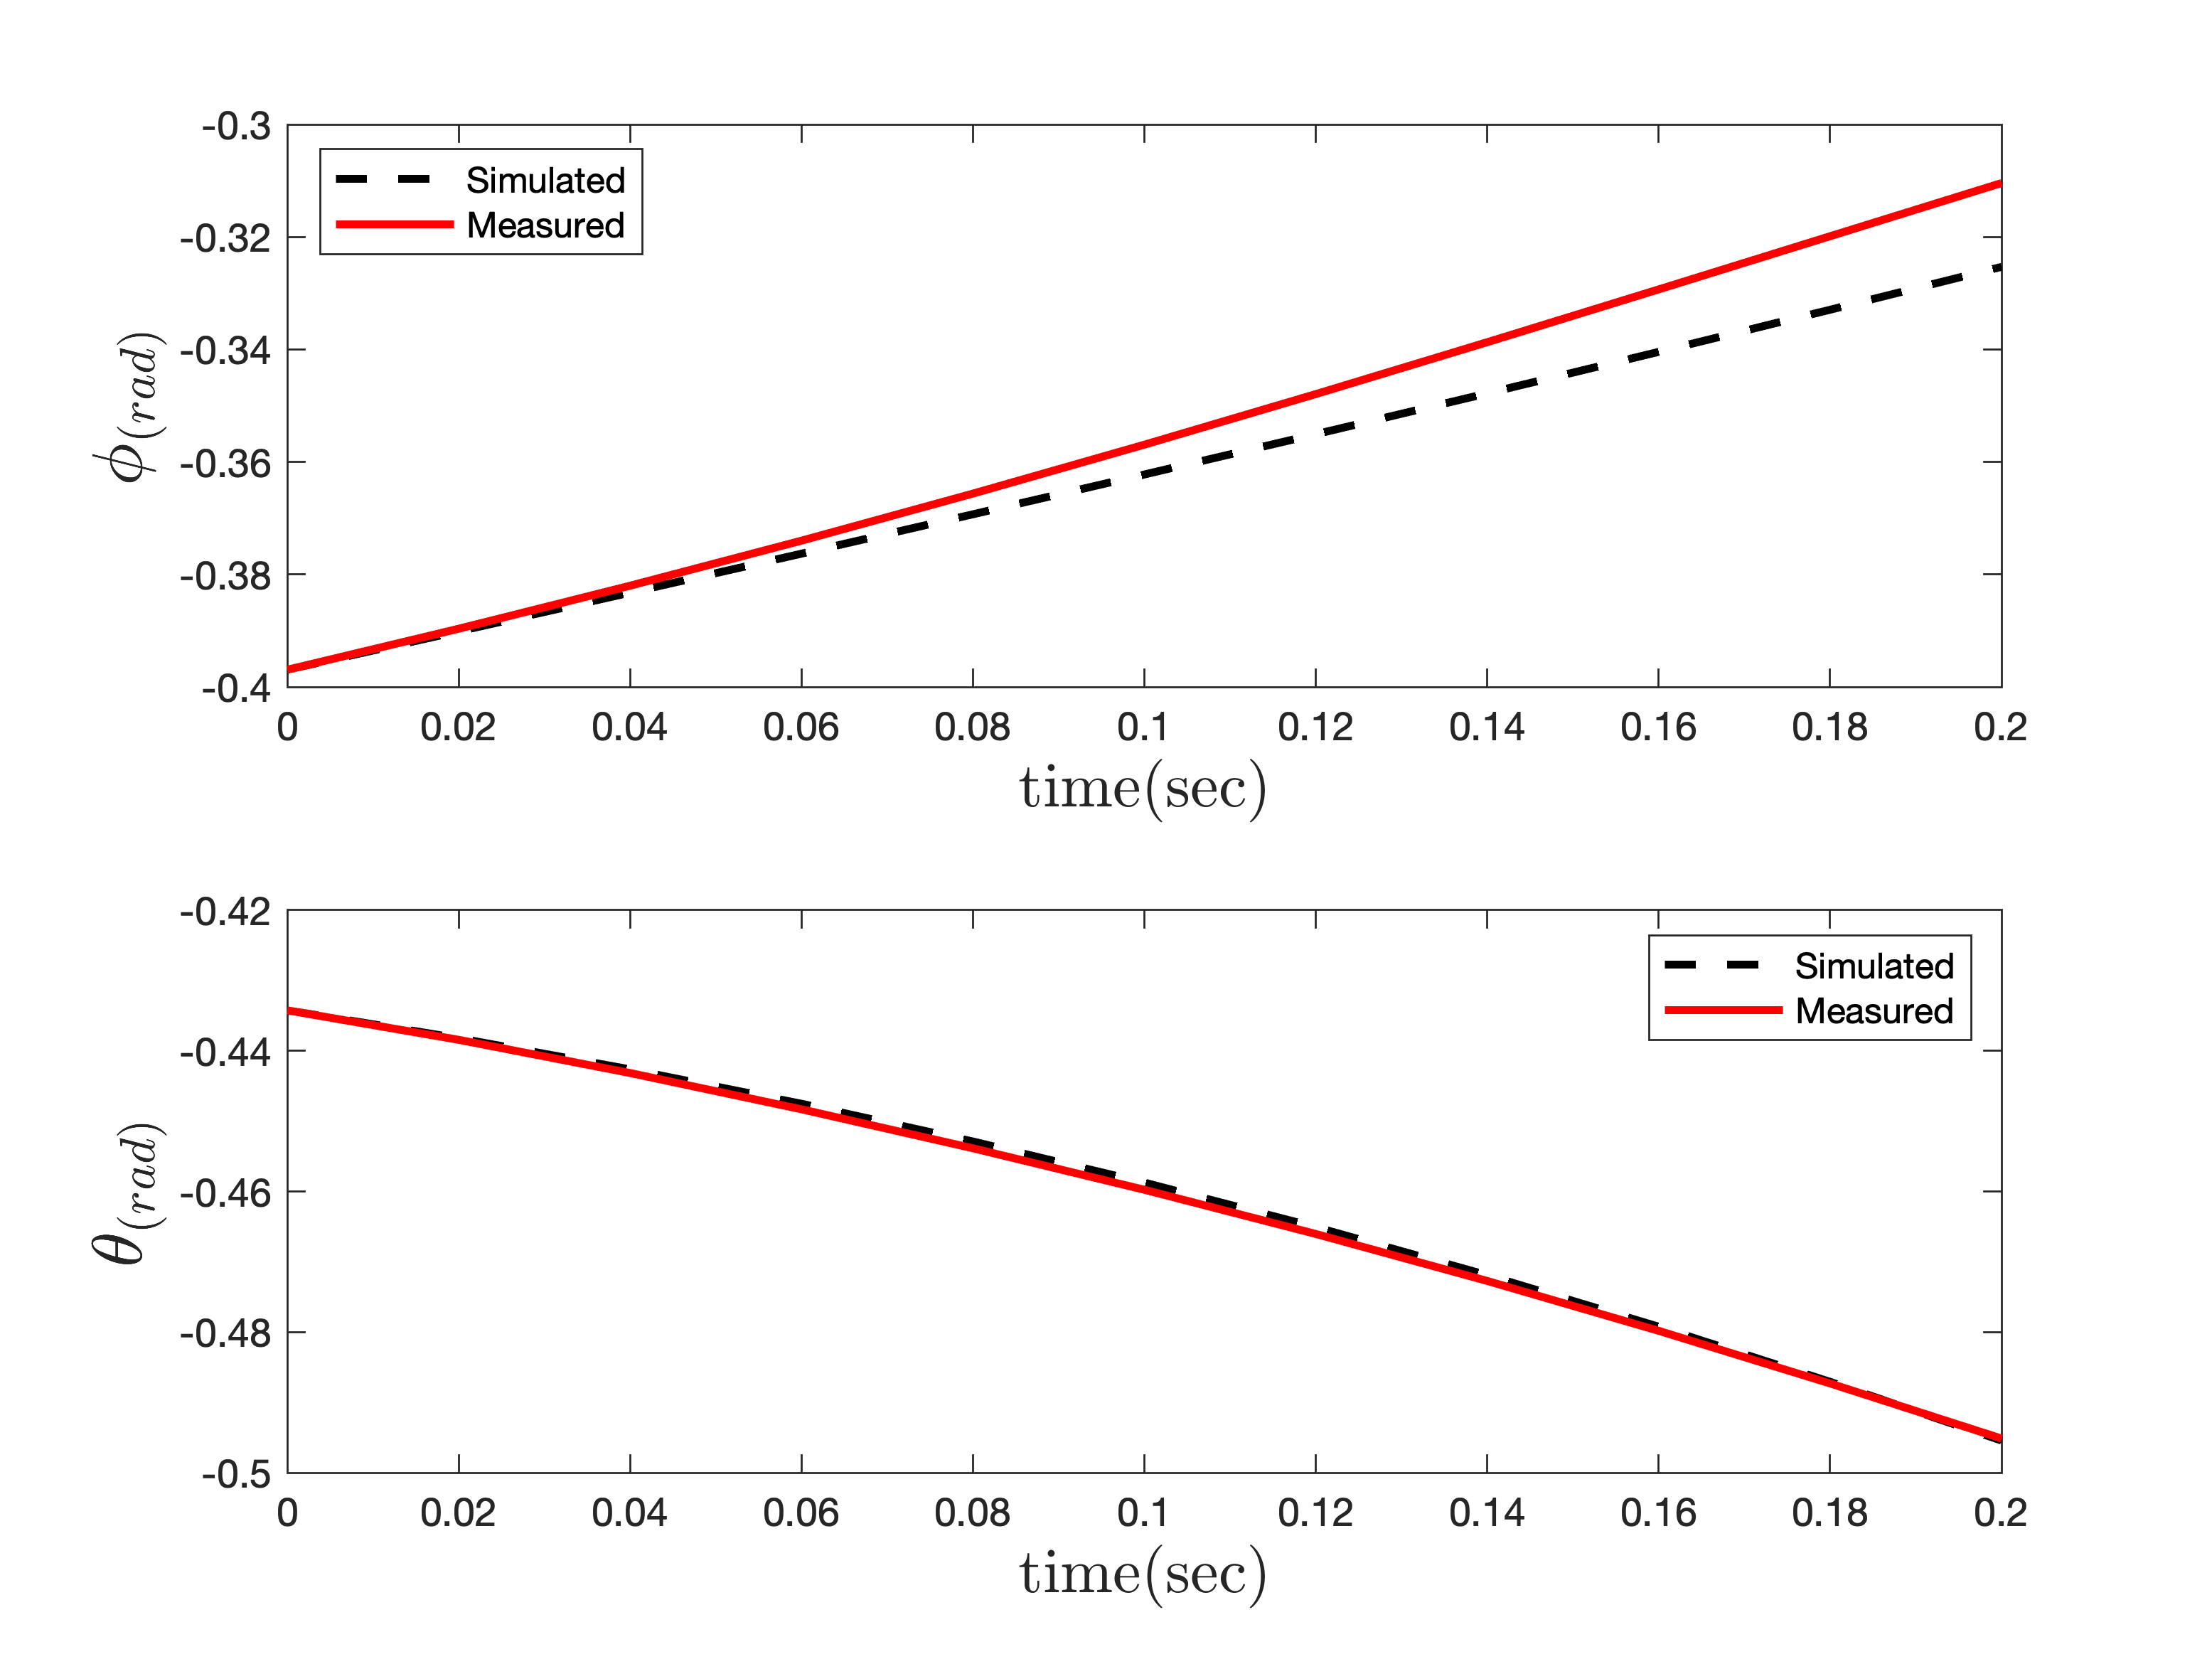
\includegraphics[width=12cm]{../Figures/RCP/roll_pitch_parameter_estimation/RCP_roll_pitch_S7.png}
%	\centering
%	\caption{مقايسه وضعیت استند در  آزمايش ششم و شبیه‌سازی، پس از تخمین پارامترهای کانال رول-پیچ}
%	\label{roll_pitch_ps7}
%\end{figure}



در این قسمت اصلاح پارمترهای مربوط به اثر متقابل کانال‌های رول و پیچ بر یکدیگر انجام شده‌است.



\begin{figure}[H]
	\centering
	\subfigure[کانال رول]{
		\centering
		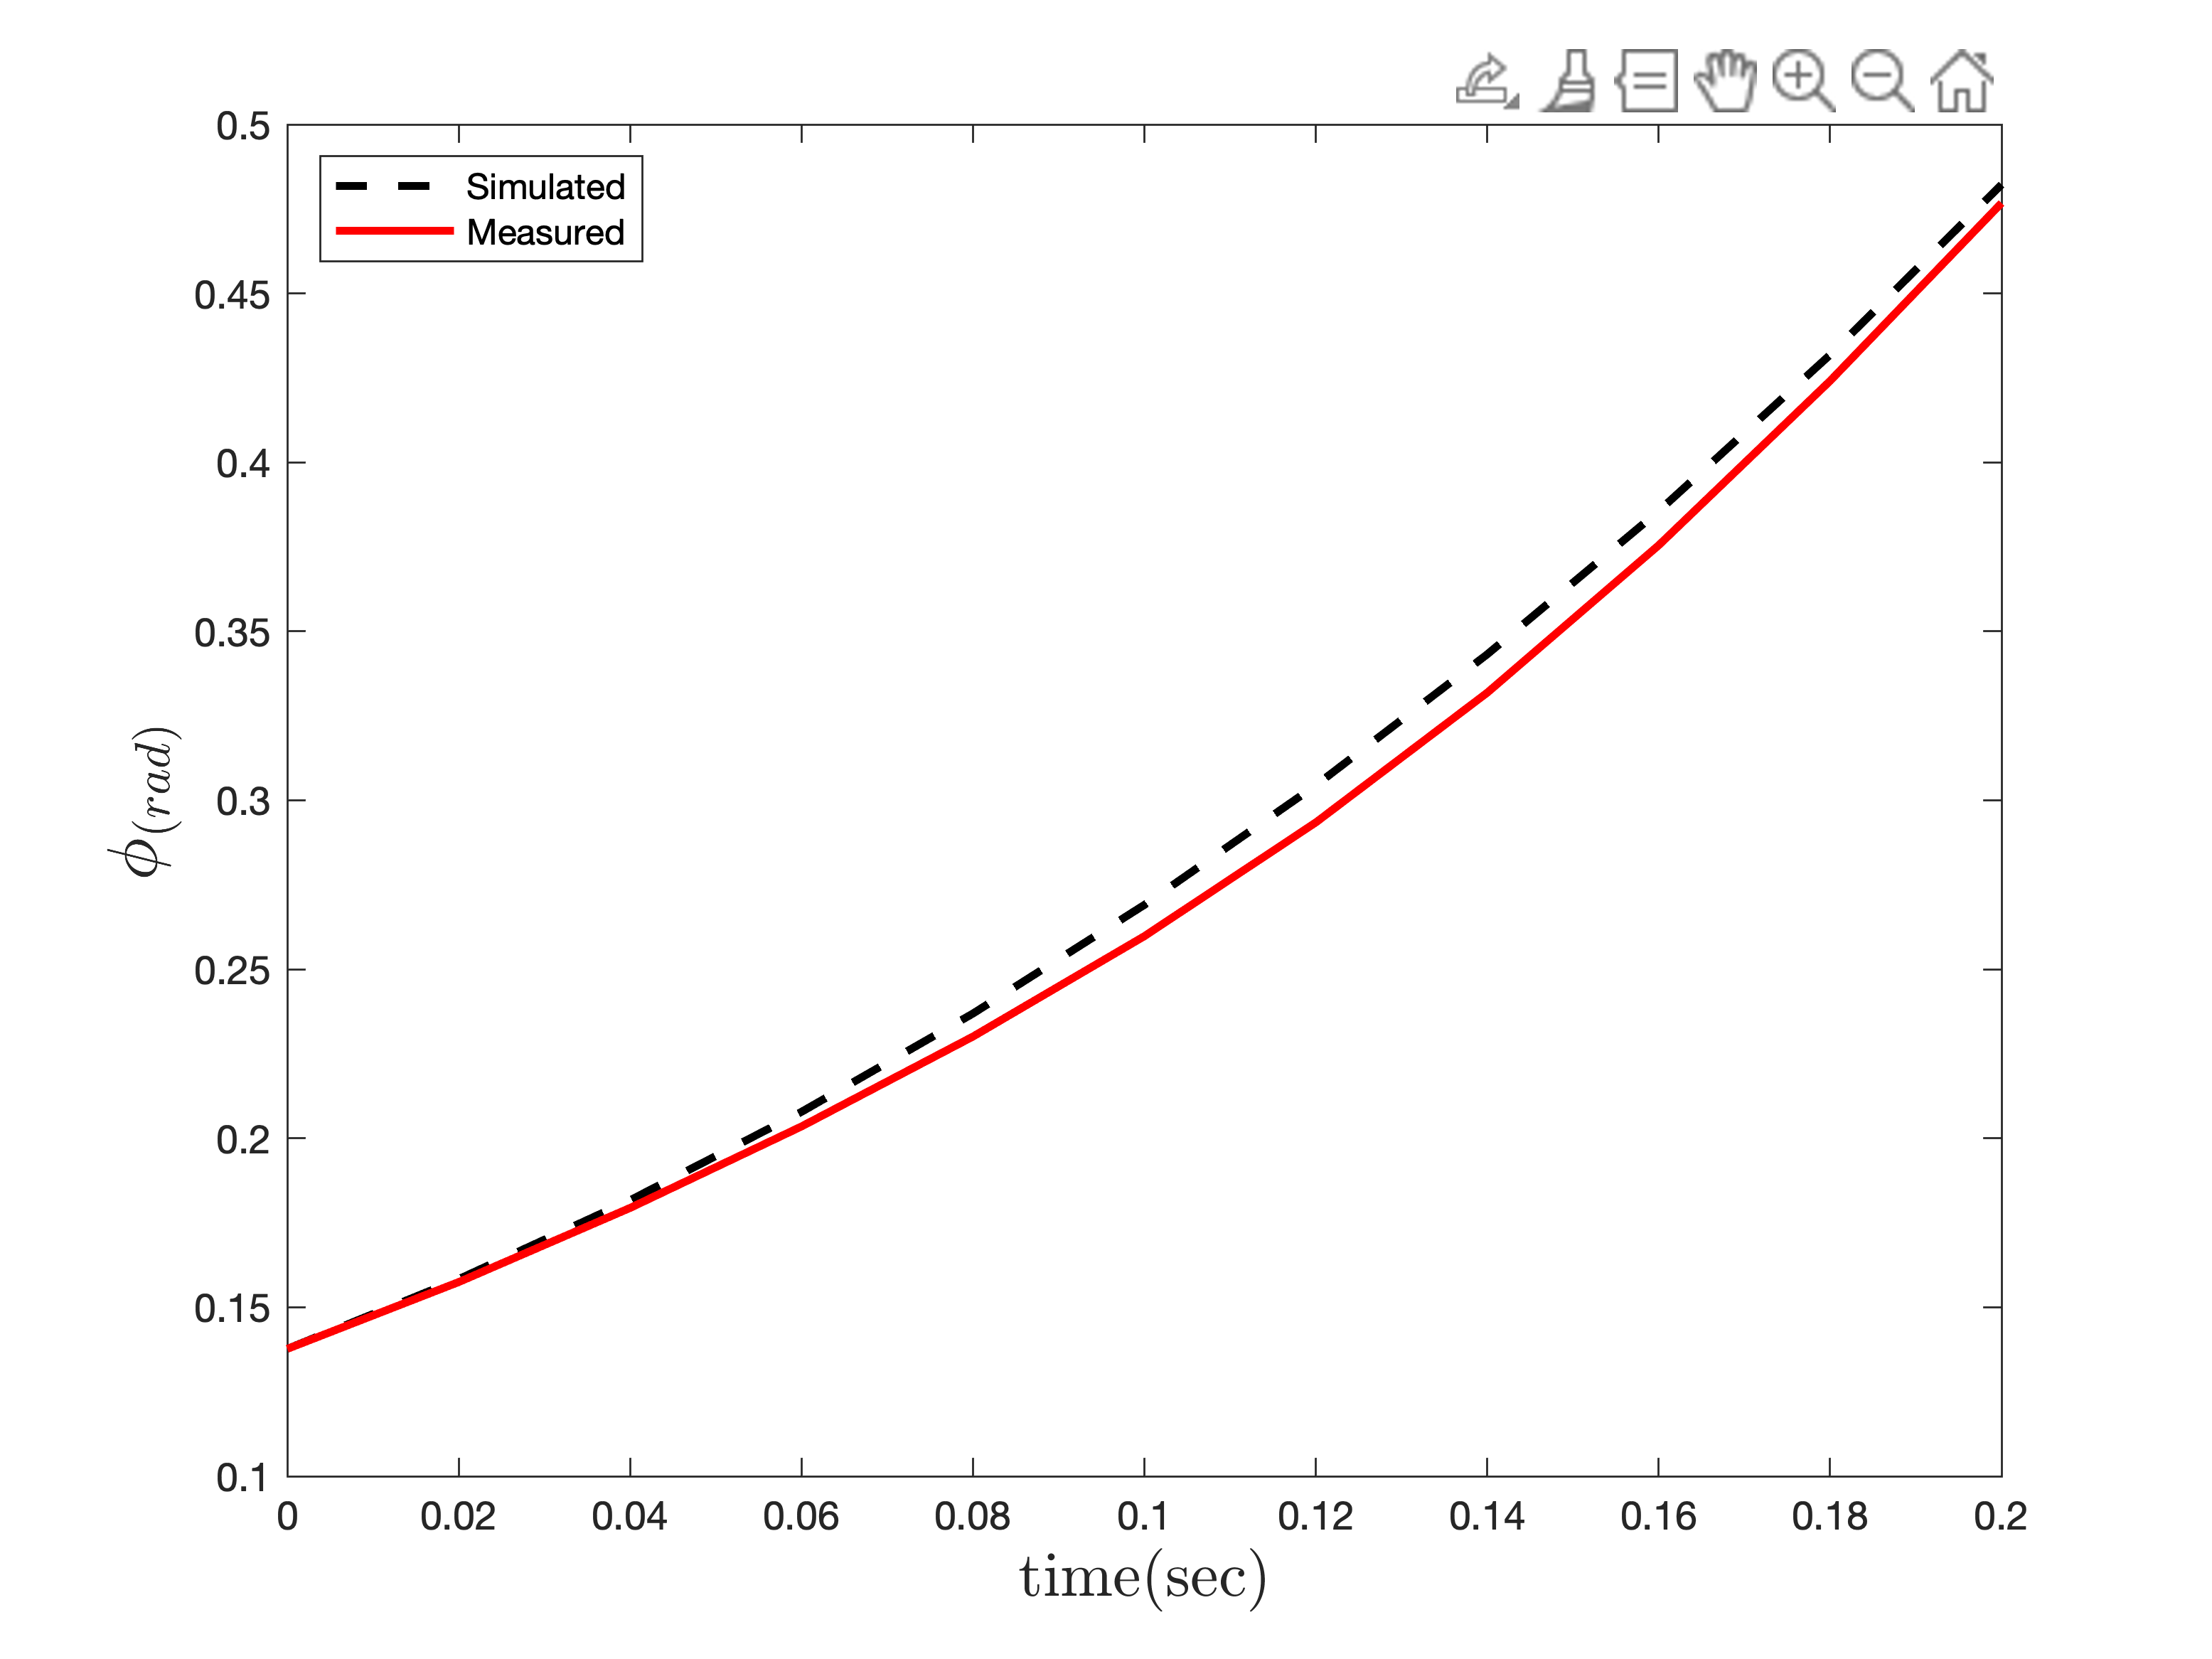
\includegraphics[width=.48\linewidth]{../Figures/RCP/roll_pitch_parameter_estimation/RCP_roll.png}
	}
	\subfigure[کانال پیچ]{
		\centering
		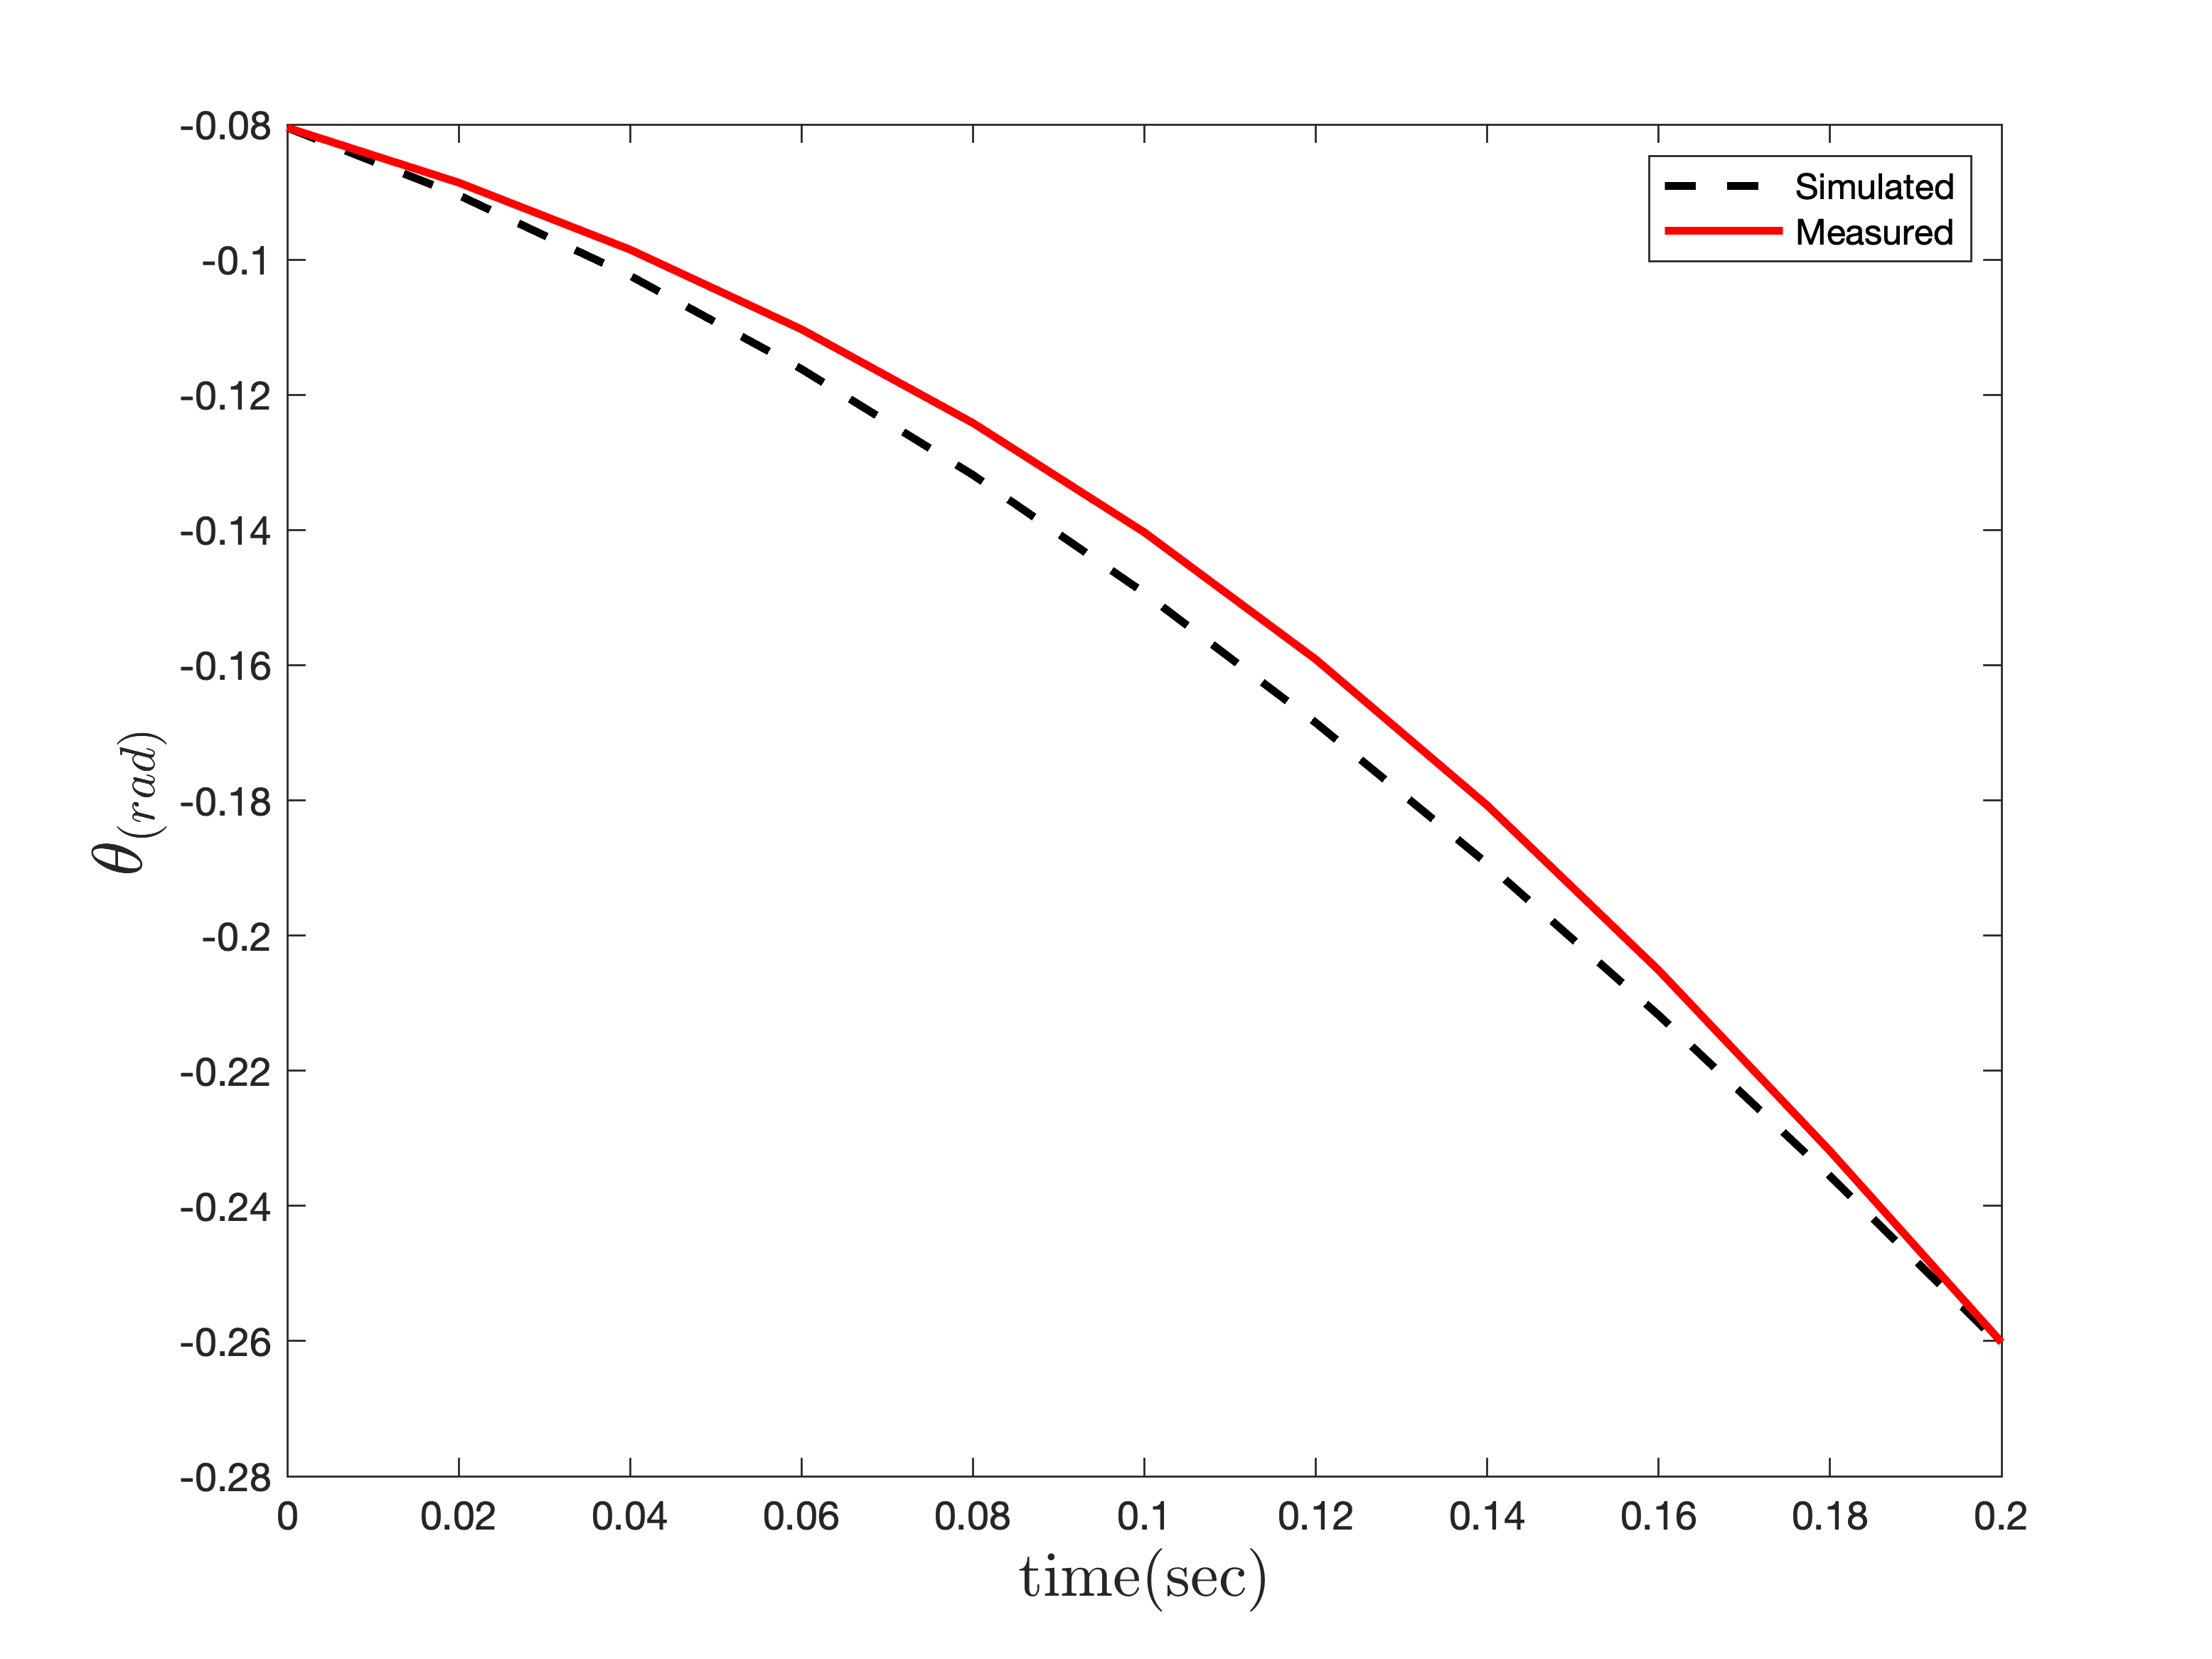
\includegraphics[width=.48\linewidth]{../Figures/RCP/roll_pitch_parameter_estimation/RCP_pitch.png}
	}
	\caption{مقايسه وضعیت کانال رول-پیچ در شبیه‌سازی و واقعیت}
%	\label{roll_pitch_ps4}
\end{figure}

\vspace{1.5cm}
\begin{table}[H]
	\begin{center}
		\begin{tabular}{ccc}\hline
	پارامتر & مقدار اولیه  & مقدار بعد از اصلاح
	\\ \hline
	$A_4$  & $0.0015$ & $0.0020$ \\
	$B_4$  & $-0.0015$ & $-0.0027$ \\ \hline
\end{tabular}
	\end{center}
\caption {مقايسه پارامترهای کانال رول-پیچ قبل و بعد از اصلاح}
\end{table}


